%
% $Id: $
%
%
% Compilar a .pdf con LaTeX (pdflatex)
% Es necesario instalar Beamer (paquete latex-beamer en Debian)
%

%
% Gr�ficos:
% Los gr�ficos pueden suministrarse en PNG, JPG, TIF, PDF, MPS
% Los EPS deben convertirse a PDF (usar epstopdf)
%

\documentclass{beamer}
\usetheme{Warsaw}
\usebackgroundtemplate{
\includegraphics[width=\paperwidth]{format/libresoft-bg-soft.png}}
\usepackage[spanish]{babel}
\usepackage[latin1]{inputenc}
\usepackage{graphics}
\usepackage{amssymb} % Simbolos matematicos

%\definecolor{libresoftgreen}{RGB}{162,190,43}
%\definecolor{libresoftblue}{RGB}{0,98,143}

%\setbeamercolor{titlelike}{bg=libresoftgreen}

%% Metadatos del PDF.
\hypersetup{
  pdftitle={Introduction to Libre Software / Master on Libre Software (URJC)},
  pdfauthor={Jesus M. Gonzalez-Barahona},
  pdfcreator={GSyC/LibreSoft, Universidad Rey Juan Carlos},
  pdfproducer=PDFLaTeX,
  pdfsubject={Introduction},
}
%%

%\includeonly{presentation}
%\includeonly{introduction}
%\includeonly{history}
\includeonly{consequences}
%\includeonly{public_administrations}
%\includeonly{trials}
%\includeonly{myths}

\AtBeginSection[]
{
\begin{frame}<beamer>
\begin{center}
{\Huge \insertsection}
\end{center}
\end{frame}
}

\begin{document}

\title{Introduction to Libre Software}
\subtitle{Master on Libre Software (URJC) \\
\url{http://master.libresoft.es}}
\author{Jesus M. Gonzalez-Barahona}
\institute{jgb@gsyc.es \\
GSyC/LibreSoft, Universidad Rey Juan Carlos}

\date{September 2010}

\frame{
\maketitle
\begin{center}

\includegraphics[width=6cm]{format/gsyc-urjc}
\end{center}
}


% Si el titulo o el autor se quieren acortar para los pies de p�gina
% se pueden redefinir aqu�:
%\title{Titulo corto}
%\author{Autores abreviado}


%% LICENCIA DE REDISTRIBUCION DE LAS TRANSPAS
\frame{
~
\vspace{3cm}

\begin{flushright}
\copyright 2000-2010 Jesus M. Gonzalez-Barahona. \\

Some rights reserved. \\
This document is distributed under the \\
Creative Commons Attribution-ShareAlike 3.0 licence, \\
available in \\
\url{http://creativecommons.org/licenses/by-sa/3.0}

The original version of this document is available at \\
\url{http://master.libresoft.es}
\end{flushright}
}
%%

%% presentation.tex
%%
%% Presentation of the course ``Master Thesis" of the Official Master on Libre Software (URJC)
%% http://master.libresoft.es
%%

%%---------------------------------------------------------------------
%%---------------------------------------------------------------------

\section{Presentation of the Master Thesis Course}

%%---------------------------------------------------------------

\begin{frame}
\frametitle{Administrative data}

\begin{itemize}
\item Both semesters, 12 ECTS credits
\item Teachers:
  \begin{itemize}
  \item Gregorio Robles (grex at gsyc.urjc.es)
  \item Jesus M. Gonzalez-Barahona (jgb at gsyc.urjc.es)
  \item Departamento de Sistemas Telem�ticos y Computaci�n (GSyC)
  \item Rooms 109 and 120 Departamental II (M�stoles campus)
  \item Room 103 Biblioteca (Fuenlabrada campus)
  \end{itemize}
\item Schedule: see Calendar
\item Sessions:
  \begin{itemize}
  \item Classroom 215, Aulario II, Fuenlabrada campus
  \end{itemize}
\item Moodle course (please, join it as soon as possible): \\
  \url{http://docencia.etsit.urjc.es/moodle/course/view.php?id=134}
\end{itemize}
\end{frame}

%%---------------------------------------------------------------

\begin{frame}
\frametitle{Goals}

Primary Goal: 
To apply the lessons and practices learned in this master
to a real problem

Secondary goal
To do it in one term

\end{frame}

%%---------------------------------------------------------------


\begin{frame}
\frametitle{Evaluation}

\begin{itemize}
\item 
\end{itemize}

\end{frame}

%%---------------------------------------------------------------

\begin{frame}
\frametitle{}

\begin{itemize}
\item 
\end{itemize}

\end{frame}

%%---------------------------------------------------------------

\begin{frame}
\frametitle{}

\begin{itemize}
\item 
\end{itemize}

\end{frame}

%%---------------------------------------------------------------

\begin{frame}
\frametitle{}

\begin{itemize}
\item 
\end{itemize}

\end{frame}


%%---------------------------------------------------------------

\begin{frame}
\frametitle{Some references}

\begin{itemize}
\item  \\
  \url{}
\item Introduction to libre software (book) \\
  \url{http://curso-sobre.berlios.de/introsobre}
\end{itemize}

\end{frame}

%% introduction.tex
%%
%% Introduction to the course ``Economic aspects'' of the
%%   Official Master on Libre Software (URJC)
%%   http://master.libresoft.es

%%---------------------------------------------------------------------
%%---------------------------------------------------------------------
\section{Introduction and motivation}

%%---------------------------------------------------------------

\begin{frame}
\frametitle{The growth of libre software (1)}

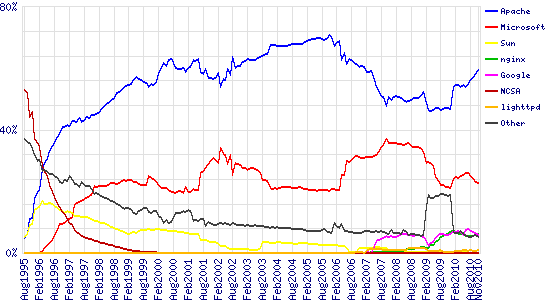
\includegraphics[height=6cm]{webservers-share-2010-11}

\begin{flushright}
Netcraft Survey, November 2010 \\
{\small \url{http://news.netcraft.com/archives/2010/11/05/november-2010-web-server-survey.html}}
\end{flushright}
\end{frame}

%%---------------------------------------------------------------

\begin{frame}
\frametitle{The growth of libre software (2)}

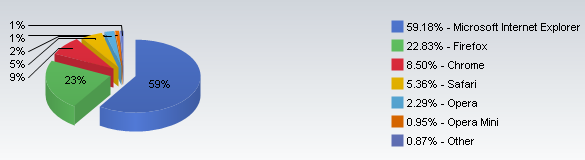
\includegraphics[height=3.5cm]{webbrowsers-share-2010-10}

\begin{flushright}
Net Market Share Report, October 2010 \\
{\small \url{http://www.netmarketshare.com/}}
\end{flushright}
\end{frame}

%%---------------------------------------------------------------

\begin{frame}
\frametitle{The growth of libre software (3)}

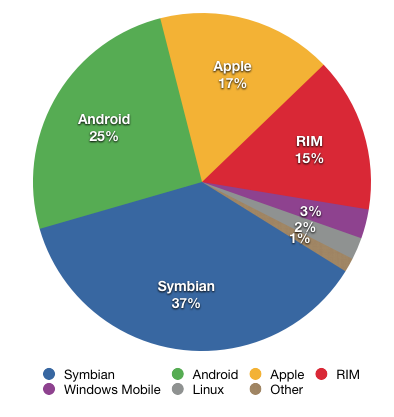
\includegraphics[height=5cm]{smartphone-share-gartner-2010-q3}

\begin{flushright}
Competitive Landscape: Mobile Devices, 3Q10 (Gartner)\\
Worldwide smartphone sales, 3rd Q 2010 \\
{\small \url{http://www.gartner.com/it/page.jsp?id=1466313}} \\
(graph from Wikimedia Commons)
\end{flushright}
\end{frame}


%%---------------------------------------------------------------

\begin{frame}
\frametitle{The adoption of libre software (1)}

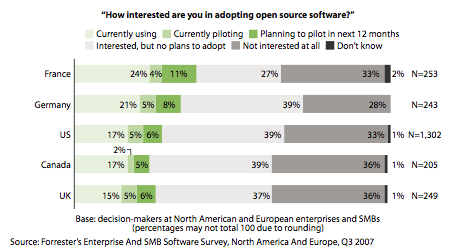
\includegraphics[height=5cm]{adoption-interest-forrester-2007-q3}

\begin{flushright}
Open Source Adoption: Notes From The Field \\
(Forrester, July 2008) \\
{\small \url{http://www.forrester.com/rb/Research/open_source_adoption_notes_from_field/q/id/46279/t/2}} 
\end{flushright}
\end{frame}

%%---------------------------------------------------------------

\begin{frame}
\frametitle{The adoption of libre software (2)}

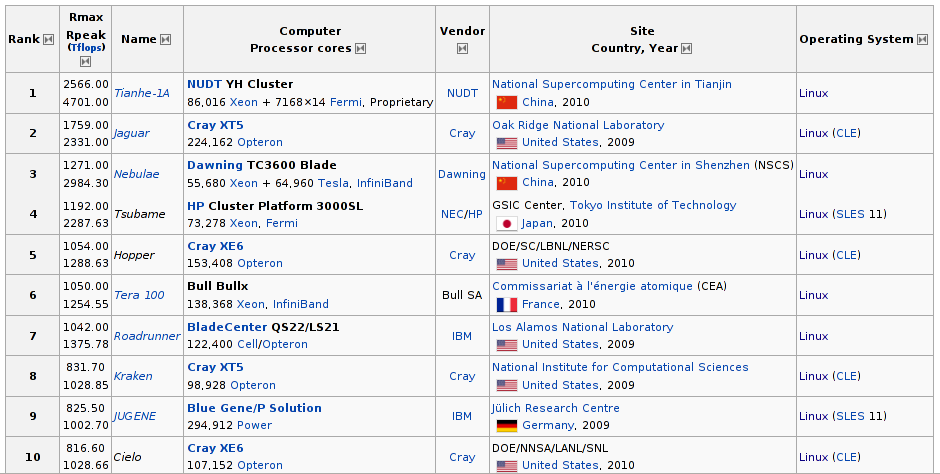
\includegraphics[height=6cm]{top-10-supercomputers-2010-11}

\begin{flushright}
36th TOP500 List (November 2010) \\
{\small \url{http://www.top500.org} \url{http://en.wikipedia.org/wiki/TOP500}} 
\end{flushright}
\end{frame}

%%---------------------------------------------------------------

\begin{frame}
\frametitle{The adoption of libre software (3)}

\begin{center}
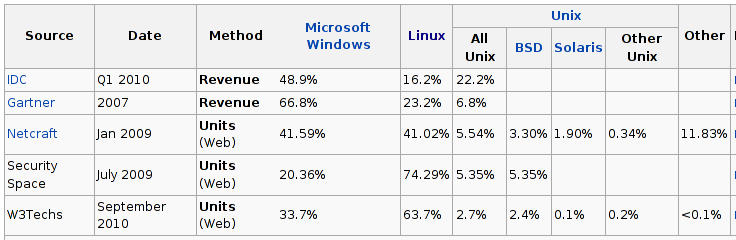
\includegraphics[height=4cm]{server-os-share-2010}
\end{center}

\begin{flushright}
Server market share, operating systems (Wikipedia) \\
{\footnotesize \url{http://en.wikipedia.org/wiki/Usage_share_of_operating_systems}} 
\end{flushright}
\end{frame}

%%---------------------------------------------------------------

\begin{frame}
\frametitle{The adoption of libre software (4)}

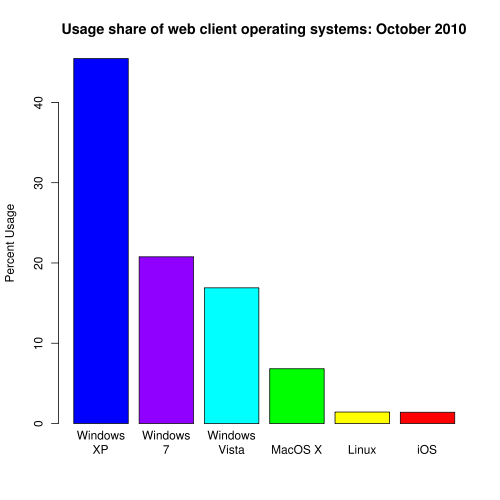
\includegraphics[height=6cm]{desktop-os-marketshare-2010-10}

\begin{flushright}
Usage share of web client operating systems \\
(Wikipedia, October 2010, median of usage studies) \\
{\small \url{http://en.wikipedia.org/wiki/Usage_share_of_desktop_operating_systems}} 
\end{flushright}
\end{frame}

\end{frame}


%
% $Id: $

\section{History of libre (free, open source) software}

%%---------------------------------------------------------------

\begin{frame}
\frametitle{Before 1970s}

\begin{itemize}
\item Software was born libre
\item Source code was shared by developers
\item Software was a kind of add-on to hardware
\item Communities of users, promoted by vendors
\item No specific market for software: vendor catalog
\end{itemize}
\end{frame}

\begin{frame}
\frametitle{1970s, early 1980s}

\begin{itemize}
\item Richard Stallman, GNU, FSF.
  \begin{itemize}
  \item Legal (GPL) and philosophical foundations.
  \item Basic infrastructure: text editor (Emacs), compiler (GCC),
    debugger (GDB), etc.
  \item Goal: building a complete system, alternative to Unix.
  \item Structured work, with clear goals.
  \end{itemize}
\item Isolated efforts: TeX, Spice, etc.
\end{itemize}
\end{frame}

 %%---------------------------------------------------------------

 \begin{frame}
 \frametitle{1970s, early 1980s (2)}

 \begin{itemize}
 \item Berkeley CSRG:
   \begin{itemize}
   \item Importance of sharing source code (``original'' Unix culture),
   \item Limited by ATT license (but not from a practical point of
     view, everyone had it).
   \item Focus on the operating system (kernel, utilities, etc.)
   \item Used in many proprietary software (SunOS, Ultrix, etc.)
   \end{itemize}
 \item Early Internet:
   \begin{itemize}
   \item Reference implementations, available for everyone.
   \item The Net as a tool for cooperation (News, ftp, email).
   \item User community provides the best support.
   \end{itemize}
 \end{itemize}

 \end{frame}

 %%---------------------------------------------------------------

 \begin{frame}
 \frametitle{Late 1980s, early 1990s}

 \begin{itemize}
 \item Complete environments around Unix (SunOS, Solaris, etc.):
   \begin{itemize}
   \item Many applications are the best ones in their field (Unix
     utilities, GCC compiler, etc.)
   \item Specially interesting: X~Window.
   \item Only a kernel is missing...
   \end{itemize}
 \item 386BSD, NetBSD, FreeBSD, OpenBSD:
   \begin{itemize}
   \item Bill Jolitz builds the parts missing in the kernel.
   \item Quickly afterwards: complete systems, similar to SunOS in
     functionality.
   \item BSD license, can be redistributed as proprietary software.
   \end{itemize}
 \end{itemize}

 \end{frame}


 %%---------------------------------------------------------------

 \begin{frame}
 \frametitle{Late 1980s, early 1990s (2)}

 \begin{itemize}
 \item GNU/Linux:
   \begin{itemize}
   \item Linus Torvalds builds his ``libre Minix''.
   \item Hundreds of developers jump on it, integrating GNU software.
   \item Porting of applications, new applications...
   \item Most code under GPL: remains libre after redistribution
   \item One kernel, many distributions (Slackware, Debian, RedHat,
     Suse, etc.).
   \item Large ``popular'' success.
   \end{itemize}
 \end{itemize}

 \end{frame}

 %%---------------------------------------------------------------

 \begin{frame}
 \frametitle{Late 1990s}

 \begin{itemize}
 \item Netscape announcement.
 \item GNU/Linux and FreeBSD compete with Windows NT.
 \item Closer and closer to the ``regular'' user: KDE, GNOME.
 \item GNU/Linux enters Universities (and student's homes).
 \item Best option is libre in many niches (Apache,
   Internet infrastructure, XFree, GCC, Gnat).
 \item Companies such as RedHat obtain venture capital.
 \item Media starts to pay attention to libre software.
 \item Large corporations (Corel, Apple, IBM) study how to deal with
   libre software.
 \end{itemize}

 \end{frame}

%%---------------------------------------------------------------

\begin{frame}
  \frametitle{Early 2000s}

  \begin{itemize}
  \item Libre software is close to be ready for the desktop
    (GNOME 2.x, KDE 3.x, OpenOffice), and it is easy to install by
    end-users.
  \item Libre software enters the strategy of large corporations (IBM,
    HP, Sun).
  \item Some others (such as Microsoft) prefer an strategy of partial
    clash.
  \item Funding difficulties due to the dotcom crisis.
  \item Penetration in public administrations and large corporations
    starts.
  \item Large increase of number of developers, quantity of available
    libre software, etc.
  \end{itemize}

\end{frame}


%%---------------------------------------------------------------

\begin{frame}
  \frametitle{Early 2000s (2)}

  \begin{itemize}
  \item A new research field studies libre software: path open to
    the understanding of how it works
  \item First effects of location independence: countries in the edges
    start to show interesting developments
  \item Some markets, some sectors, consider libre software as a
    ``natural'' option.
  \item Legal environment is changing: will it became hostile to libre
    software?
  \end{itemize}

\end{frame}


%%---------------------------------------------------------------

\begin{frame}
  \frametitle{Late 2000s}

  \begin{itemize}
  \item Libre software is strategic for many companies (ej: Google).
  \item Complete application suites for many environments.
  \item Companies testing new collaboration models (ej: OW2, Morfeo).
  \item New business models, models for new business.
  \item Libre software as an enabler in many industries.
  \item Libre software is becoming ``business as usual''.
  \end{itemize}

\end{frame}

%%---------------------------------------------------------------

\begin{frame}
  \frametitle{The future: an obstacle race?}

  Future evolution of libre software can find some obstacles:

  \begin{itemize}
  \item FUD (fear, uncertainty, doubt) techniques: up to know have
    caused little harm.
  \item ``Dissolution'' (models which can be mistaken with libre
    software): community split, loss of model advantages
  \item Ignorance (loss of vision): why is libre software interesting?
  \item Legal barriers: software patents, DRM, etc.
  \end{itemize}

\end{frame}

%%---------------------------------------------------------------

\begin{frame}
  %\frametitle{}

  \begin{center}
  {\LARGE \bf How will libre software status be in 10 years?}
  \end{center}

\end{frame}

%%
%% Consequences of the libre software model
%%
%% Master on libre software
%% http://master.libresoft.es

\section{Some consequences of the model}

%%---------------------------------------------------------------

\begin{frame}
\frametitle{Consequences for the software industry}

The software business is changing upside down (still slowly, but
gaining momentum):

\begin{itemize} 
\item Traditional software ``manufacturers'' will have to reinvent
  themselves completely (no more per-copy incomes).
\item A whole new industry (based in support and libre development)
  will be needed as libre software gains market acceptance.
\item It allows for (and encourages) competition in support, and even
  in the evolution of a piece of software.
\item Users are benefited in several ways. Therefore, big pressure
  from end-users (including big companies) to switch to libre software.
\end{itemize}

\end{frame}

%%---------------------------------------------------------------

\begin{frame}
\frametitle{Some specific impacts}

\begin{itemize} 
\item Cost: cost model radically different from proprietary software
\item Openess: can be modified, can be inspected, can be studied
\item Distribution: new distribution channels, new methods
\item Development: ``surprising'' development models
\item Maintenance and support: true competition
\end{itemize}

Mixture of two powerful mechanisms:

\begin{itemize}
\item Competition (using the same souce base)
\item Cooperation (even non-voluntary)
\end{itemize}

\end{frame}

%%---------------------------------------------------------------

\begin{frame}
\frametitle{How libre software affects...}

\begin{itemize}
\item End user (individual or company)
\item Developer (or software producer)
\item Integrator
\item Maintenance and services
\end{itemize}
\end{frame}


%%---------------------------------------------------------------

\begin{frame}
\frametitle{End user}

End users can forget about...

\begin{itemize}
\item ...company monopolies \\
  (real competition, best products and services)
\item ...producer `reliability' \\
  (future path ensured by product acceptance, source code availability, community dynamics)
\item ...decision taking with few elements \\
  (software can be tested in real environments, with near-zero cost)
\item ...dependence on provider's strategies \\
  (many providers, community strategies, strategies follow clients)
\item ...black boxes \\
  (no longer ``blind confidence'')
\end{itemize}
\end{frame}

%%---------------------------------------------------------------

\begin{frame}
\frametitle{End user (2)}

What if users could...

\begin{itemize}
\item ...adapt/customize the product at will?
\item ...have the latest release with (very) low cost?
\item ...fix all the problems (or hire someone to fix them)?
\item ...decide on the future evolution of the product?
\item ...contract the (complete) integration of the best products in a given area?
\item ...buy complete auditing for each product by independent third parties?
\end{itemize}
\end{frame}

%%---------------------------------------------------------------

\begin{frame}
\frametitle{End user (3)}

\begin{center}
{\LARGE A large portion of the control moves to the user \\
(from the producer of the software)}
\end{center}
\end{frame}

%%---------------------------------------------------------------

\begin{frame}
\frametitle{Other general issues for (large) end users}

\begin{itemize}
\item Libre software is not necessarily better or worse. It is 
  just different
\item In several niches, we have already excelent products and
  companies supporting them.
\item In many cases, the most cost-effective way of producing
  software.
\item Special advantages when there is interest in long-term life
  cycles, vendor independence, multiplatform support, adaption to
  evolving technologies.
\item If a powerful enough user (or group of users) needs to drive the
  technology, this is probably the best way to go.
\item Many things can be done to promote a competitive
  libre software industry in a given niche. Many benefits
  are derived of such a promotion.
\end{itemize}
\end{frame}

%%---------------------------------------------------------------

\begin{frame}
\frametitle{Developer (or software producer)}

Libre software changes the rules of the game:

\begin{itemize}
\item Opportunities for competing while being small
\item Easier (and cheaper) to acquire front-wave technology
\item Can take advantage of the work of your competitors (but they can do the same!)
\item External contributors can be found (in many cases, at a fraction of the usual cost, because of win-win relationships)
\item Distribution channels are cheaper, and truly global
\item Feasible to become reference application in a niche
\end{itemize}
\end{frame}


%%---------------------------------------------------------------

\begin{frame}
\frametitle{Developer (or software producer) (2)}

Where does the money come from? (sustainability)
\begin{itemize}
\item The producer enjoys the best knowledge about its product
\item Producer can be the ``most visible point'', if image is cared of
\item Custom-made development, modifications, customizations
\item ``In depth'' support (bug fixing, preference in access to new releases, new features)
\end{itemize}

\begin{center}
{\large Assuming there is a need for a software product \\
  and there is money ready for supporting that need \\
  some developer/producer will benefit from the situation \\
  (if both parts are put in contact)
}
\end{center}
\end{frame}


%%---------------------------------------------------------------

\begin{frame}
\frametitle{Integrator}

Maybe the best placed actor:

\begin{itemize}
\item All libre software products available (without the constraints of proprietary licences!)
\item If products ``don't fit'' you can adapt them (source code is available, interoperability is always possible)
\item Pieces of products, or full products, or anything in the middle, can be integrated
\item No more black boxes: everything is transparent 
\end{itemize}

\begin{center}
{\large They can build on top of the work of others, with similar constraints and possibilities to those others}
\end{center}
\end{frame}


%%---------------------------------------------------------------

\begin{frame}
\frametitle{Services and maintenance}

\begin{itemize}
\item Similar conditions than the producer
\item Competition in the maintenance business
\item Added-value of services is better appreciated (the base cost of the program is low)
\item Good knowledge of the state of the art is important (good idea to have good links with libre software projects)
\item New business models: advising on releases and combination of programs, information about new development, project management, etc.
\item The most diverse and massive kind of business right now
\end{itemize}
\end{frame}

%%---------------------------------------------------------------

\begin{frame}
\frametitle{Some conclusions}

\begin{itemize}
\item Libre software changes the rules of the game
\item It is important to understand (and get advantage) of those rules
\item Still learning effects and mechanisms
\item Many opportunities to discover new effects, and take advantage of them
\end{itemize}
\end{frame}

%%---------------------------------------------------------------

\begin{frame}
\frametitle{To probe further}

\begin{itemize}
\item ``SME Guide to Free Software'', by Carlo Daffara \\
  \url{http://guide.flossmetrics.org}
\end{itemize}
\end{frame}

%% public_administrations.tex
%%
%% Presentation of the relationship of public administrations and free software for the Official Master on Libre Software (URJC)
%% http://master.libresoft.es
%%

%%---------------------------------------------------------------------
%%---------------------------------------------------------------------

\section{Public Administrations and Libre Software}


%%%%%%%%%%%%%%%%%%%%%%%%%%%%%%%%%%%%%%%%%%%%%%%%%%%%%%%%%%%%%%%%%%%%%%%

%%---------------------------------------------------------------

\begin{frame}
\frametitle{Impacto en las administraciones p�blicas}

\begin{itemize}
\item Aprovechamiento m�s adecuado de recursos: m�s impacto para la
  misma inversi�n (ejemplo: localizaci�n)
\item Fomento del tejido tecnol�gico local
\item Independencia del proveedor
\item Adaptaci�n a las necesidades exactas
\item Escrutinio p�blico (en seguridad, rendimiento, etc.)
\item Disponibilidad a largo plazo
\end{itemize}

\end{frame}

%%---------------------------------------------------------------

\begin{frame}
\frametitle{Dificultades de adopci�n}

\begin{itemize}
\item Desconocimiento y falta de decisi�n pol�tica
\item Poca adecuaci�n de los mecanismos de contrataci�n
\item Falta de estrategia de implantaci�n
\item Escasez o ausencia de productos libres en ciertos segmentos
\end{itemize}

\end{frame}

%%---------------------------------------------------------------

\begin{frame}
\frametitle{Actuaciones de las administraciones p�blicas}

\begin{itemize}
\item Compra de servicios y sistemas basados en software libre
  (gen�ricos, a medida, etc.)
\item Promoci�n de la sociedad de la informaci�n (uso de software a
  gran escala)
\item Fomento de la investigaci�n
\end{itemize}

\end{frame}

%%---------------------------------------------------------------

\begin{frame}
\frametitle{Algunos escenarios ejemplo}

\begin{itemize}
\item Concurso p�blico para la adquisici�n de un juego de aplicaciones
  ofim�ticas con ciertas especificaciones
  \begin{itemize}
  \item proyecto a dos a�os,
  \item decenas o centenas de miles de puestos
  \item varios ganadores que
  compitan entre ellos por tener m�s usuarios
\end{itemize}
\item Consorcio de administraciones que contratan un software a medida
  con la condici�n de que el resultado sea software libre
  \begin{itemize}
  \item despliegue y otros servicios incluidos en el contrato
  \item otras administraciones interesadas pueden entrar en el
    consorcio o contratar por su cuenta
  \end{itemize}
\end{itemize}

\end{frame}

%%---------------------------------------------------------------

\begin{frame}
\frametitle{Algunos casos reales}

\begin{itemize}
\item Proyecto LiMux en Munich
\item Estrategia en Extremadura, basada en LinEx
\item Software libre en Brasil
\end{itemize}

\begin{flushright}
  \url{http://www.muenchen.de/Rathaus/referate/dir/limux/89256/} \\
  \url{http://www.linex.org/} \\
  \url{http://www.softwarelivre.org/}
\end{flushright}
\end{frame}


%% trials.tex
%%
%% Presentation of the trials activity for the Official Master on Libre Software (URJC)
%% http://master.libresoft.es
%%

%%---------------------------------------------------------------------
%%---------------------------------------------------------------------

\section{Description of the activity}


\begin{frame}
\frametitle{Activity: Trials - Process}

\begin{itemize}
\item Presentation of the statements (by the lecturer)
\item Preliminary voting by the jury (in favour, against, abstention)
\item Trial. Defense and attorneys will have:
\begin{itemize}
  \item 5 minutes to present their position (slides allowed)
  \item 3 minutes to rebate
\end{itemize}
\item Final voting by the jury (in favour, against, abstention)
\item Discusison (all students)
\end{itemize}

\end{frame}


\begin{frame}
\frametitle{Trial Statement \#1}

\begin{center}
\begin{LARGE}
``A new freedom should be added to the Free Software Definition:
all their derived works should alwasy be free.''
\end{LARGE}
\end{center}

\end{frame}



\begin{frame}
\frametitle{Trial Statement \#2}

\begin{center}
\begin{LARGE}
``Non-commercial software should also be considered free software.''
\end{LARGE}
\end{center}

\end{frame}



\begin{frame}
\frametitle{Trial Statement \#3}

\begin{center}
\begin{LARGE}
``Governments should act in a neutral way when releasing policies regarding
free software''
\end{LARGE}
\end{center}

\end{frame}


\begin{frame}
\frametitle{Trial: Statements}

\begin{center}
\begin{LARGE}
``A new freedom should be added to the Free Software Definition:
all their derived works should alwasy be free.''
\end{LARGE}
\end{center}
\begin{center}
\begin{LARGE}
``Non-commercial software should also be considered free software.''
\end{LARGE}
\end{center}

\begin{center}
\begin{LARGE}
``Governments should act in a neutral way when releasing policies regarding
free software''
\end{LARGE}
\end{center}

\end{frame}

%%---------------------------------------------------------------


%% myths.tex
%%
%% Presentation of the myths activity for the Official Master on Libre Software (URJC)
%% http://master.libresoft.es
%%

%%---------------------------------------------------------------------
%%---------------------------------------------------------------------

\section{Myths}


%%%%%%%%%%%%%%%%%%%%%%%%%%%%%%%%%%%%%%%%%%%%%%%%%%%%%%%%%%%%%%%%%%%%%%%

\begin{frame}

\begin{center}
\huge{``El copyleft est� en contra del derecho de autor''}
\end{center}

\end{frame}


%%%%%%%%%%%%%%%%%%%%%%%%%%%%%%%%%%%%%%%%%%%%%%%%%%%%%%%%%%%%%%%%%%%%%%%

\begin{frame}

\begin{center}
\huge{``El software libre no tiene titulares o propietarios''}
\end{center}

\end{frame}

%%%%%%%%%%%%%%%%%%%%%%%%%%%%%%%%%%%%%%%%%%%%%%%%%%%%%%%%%%%%%%%%%%%%%%%

\begin{frame}

\begin{center}
\huge{`` Las licencias libres obligan a ceder sus derechos de
autor''}
\end{center}

\end{frame}


%%%%%%%%%%%%%%%%%%%%%%%%%%%%%%%%%%%%%%%%%%%%%%%%%%%%%%%%%%%%%%%%%%%%%%%

\begin{frame}

\begin{center}
\huge{``No se puede hacer un uso comercial del software libre''}
\end{center}

\end{frame}


%%%%%%%%%%%%%%%%%%%%%%%%%%%%%%%%%%%%%%%%%%%%%%%%%%%%%%%%%%%%%%%%%%%%%%%

\begin{frame}

\begin{center}
\huge{``  El software libre y el software propietario son
incompatibles''}
\end{center}

\end{frame}


%%%%%%%%%%%%%%%%%%%%%%%%%%%%%%%%%%%%%%%%%%%%%%%%%%%%%%%%%%%%%%%%%%%%%%%

\begin{frame}

\begin{center}
\huge{`` No se pueden integrar o mezclar software libre y software propietario''}
\end{center}

\end{frame}


%%%%%%%%%%%%%%%%%%%%%%%%%%%%%%%%%%%%%%%%%%%%%%%%%%%%%%%%%%%%%%%%%%%%%%%

\begin{frame}

\begin{center}
\huge{`` Todo el software libre es igual" (en los t�rminos de la
GPL)''}
\end{center}

\end{frame}


%%%%%%%%%%%%%%%%%%%%%%%%%%%%%%%%%%%%%%%%%%%%%%%%%%%%%%%%%%%%%%%%%%%%%%%

\begin{frame}

\begin{center}
\huge{`` Las licencias libres obligan a publicar sus
modificaciones particulares''}
\end{center}

\end{frame}


%%%%%%%%%%%%%%%%%%%%%%%%%%%%%%%%%%%%%%%%%%%%%%%%%%%%%%%%%%%%%%%%%%%%%%%

\begin{frame}

\begin{center}
\huge{``El software libre no tiene responsables ni garant�as''}
\end{center}

\end{frame}


%%%%%%%%%%%%%%%%%%%%%%%%%%%%%%%%%%%%%%%%%%%%%%%%%%%%%%%%%%%%%%%%%%%%%%%

\begin{frame}

\begin{center}
\huge{``El software libre puede ser usado para el genocidio''}
\end{center}

\end{frame}


%%%%%%%%%%%%%%%%%%%%%%%%%%%%%%%%%%%%%%%%%%%%%%%%%%%%%%%%%%%%%%%%%%%%%%%

\begin{frame}

\begin{center}
\huge{``El software libre es comunista''}
\end{center}

\end{frame}


%%%%%%%%%%%%%%%%%%%%%%%%%%%%%%%%%%%%%%%%%%%%%%%%%%%%%%%%%%%%%%%%%%%%%%%

\begin{frame}

\begin{center}
\huge{``El software libre es liberal''}
\end{center}

\end{frame}


%%%%%%%%%%%%%%%%%%%%%%%%%%%%%%%%%%%%%%%%%%%%%%%%%%%%%%%%%%%%%%%%%%%%%%%

\begin{frame}

\begin{center}
\huge{``La pluralidad de licencias libres es positiva''}
\end{center}

\end{frame}


%%%%%%%%%%%%%%%%%%%%%%%%%%%%%%%%%%%%%%%%%%%%%%%%%%%%%%%%%%%%%%%%%%%%%%%

\begin{frame}

\begin{center}
\huge{``El software libre comienza con Richard Stallman''}
\end{center}

\end{frame}


%%%%%%%%%%%%%%%%%%%%%%%%%%%%%%%%%%%%%%%%%%%%%%%%%%%%%%%%%%%%%%%%%%%%%%%

\begin{frame}

\begin{center}
\huge{``El software libre es t�cnicamente superior''}
\end{center}

\end{frame}

%%%%%%%%%%%%%%%%%%%%%%%%%%%%%%%%%%%%%%%%%%%%%%%%%%%%%%%%%%%%%%%%%%%%%%%

\begin{frame}

\begin{center}
\huge{``El software libre es m�s seguro''}
\end{center}

\end{frame}

%%%%%%%%%%%%%%%%%%%%%%%%%%%%%%%%%%%%%%%%%%%%%%%%%%%%%%%%%%%%%%%%%%%%%%%

\begin{frame}

\begin{center}
\huge{``La cultura libre se opone a las grandes corporaciones''}
\end{center}

\end{frame}


%%---------------------------------------------------------------




\end{document}
